% Document setup
\documentclass[11pt]{book}

% Location of the csas-style repository: adjust path as needed
\newcommand{\locRepo}{csas-style}

% Use the style file in the csas-style repository (sr.sty)
\usepackage{\locRepo/sr}

% header-includes from R markdown entry
\usepackage{pdflscape}

% Bibliography style file
% \bibliographystyle{../csas-style/res-doc}

%%%% Commands for title page etc %%%%%

% Title
\newcommand{\rdTitle}{Evaluating the robustness of candidate management procedures in the BC sablefish (\emph{Anoplopoma fibria}) for 2019-2020.}

% French title
\newcommand{\rdTitleFr}{}

% Title short
\newcommand{\rdTitleShort}{Robustness of sablefish MPs in BC}

% Publication year
\newcommand{\rdYear}{2019}

% Publication month
\newcommand{\rdMonth}{October}

% Report number
\newcommand{\rdNumber}{nnn}

% Approver (name\\position)
\newcommand{\rdApp}{Approver Name\\
Regional Director\\
Science Branch, Pacific Region\\
Fisheries and Oceans Canada}
% \newcommand{\rdYear}{20XX}
% \newcommand{\rdAppMonth}{January}
% \newcommand{\rdAppDay}{01}
\newcommand{\rdAppDate}{January 01, 20XX}

% Branch
\newcommand{\rdBranch}{Science Branch}

% Region
\newcommand{\rdRegion}{Pacific Region}

% Address
\newcommand{\rdAddress}{\textsuperscript{1}Pacific Biological Station\\
Fisheries and Oceans Canada, 3190 Hammond Bay Road\\
Nanaimo, British Columbia, V9T 6N7, Canada\\
\textsuperscript{2}Far, far away\\
Another Galaxy}

% Phone
\newcommand{\rdPhone}{(250) 756-7208}

% Email
\newcommand{\rdEmail}{\href{mailto:csap@dfo-mpo.gc.ca}{\nolinkurl{csap@dfo-mpo.gc.ca}}}

%%%% End of title page commands %%%%%
\begin{document}

\MakeFirstPage

\hypertarget{appendix-appendices}{%
\appendix}


\hypertarget{appendix-a-updated-operating-model-components}{%
\section{Appendix A: Updated operating model components}\label{appendix-a-updated-operating-model-components}}

\hypertarget{updated-ageing-error-matrix}{%
\subsection{Updated ageing error matrix}\label{updated-ageing-error-matrix}}

The Sablefish age-structured assessment model relies on catch-at-age data to estimate the true age-composition of the population; however, observed catch-at-age data are based on otolith readings that are imperfectly known. Failure to account for errors in otolith readings may lead to smoothing estimates of age-classe, making it more difficult to detect strong recruitment years or stock-recruit relationships (Hanselman et al. \protect\hyperlink{ref-hanselman2012statistical}{2012}). Ageing errors may also bias estimates of growth parameters, maturity schedules, and natural mortality that can lead to overfishing or inaccurate yield projections (Lai and Gunderson \protect\hyperlink{ref-lai1987effects}{1987}; Tyler et al. \protect\hyperlink{ref-tyler1989implications}{1989})

To account for ageing-error we developed ageing-error matrices based on otoliths that had been read by two different readers at the DFO Pacific Biological Station ageing lab. These data account for approximately 15\% of the total otolith readings for BC Sablefish, which are read first by the primary reader and then by a secondary reader as a quality control. In the majority of cases both readers agreed (62\%) and in cases where the two readings differ (38\%), both readers conferred to resolve the discrepancy and agree on the final age assigned (Pers. Comm, B. Connors, DFO). In most cases the final age reading was that assigned by the secondary or primary reader (36\%), but in a few cases a new age was assigned (2\%).

We applied statistical models for estimating the probability of observing an age class (a) given the true age (b) based on methods described in Richards et al. (\protect\hyperlink{ref-richards1992statistical}{1992}) and Heifetz et al. (\protect\hyperlink{ref-heifetz1999age}{1999}). The model assumes a normal ageing-error distribution where the estimated standard deviation of the observed age for a true age b is based on three parameters \(\Phi = \{ \sigma_1, \sigma_A, \alpha \}\) in the form:
\begin{equation}
\sigma(b) = \left\{
    \begin{array}{ll}
        \sigma_1 + (\sigma_A - \sigma_1) \frac{1 - e^{-\alpha(b - 1)} }{1 - e^{-\alpha(A - 1)}}, & \alpha \neq 0; \\
        \sigma_1 + (\sigma_A - \sigma_1) \frac{b-1}{A-1}, & \alpha = 0.\\
    \end{array} \right.
\end{equation}
Parameters \(\sigma_1\) and \(\sigma_A\) are the standard deviations for \(b=1\) and \(b=A\), representing the minimum and maximum ages, respectively. The \(\alpha\) parameter determines the non-linearity of the function, such that\\
\(\sigma(b)\) becomes linear as \(\alpha \rightarrow 0\). The age-error matrix is defined as:
\begin{align}
q(a ~|~ b, \Phi) &= \frac{x_{ab}(\Phi)}{\sum_{a = 1}^A x_{ab}(\Phi) }; \\
x_{ab} &= \frac{1}{\sqrt{2\pi}\sigma(b)} e^{-\frac12 \left[ \frac{a-b}{\sigma(b)} \right]^2}.
\end{align}
Given that the true age of the fish is unknown, it is not possible to accurately determine bias in the age readings and whether certain age classes are more likely to be under or over-estimated. We tested 2 different approaches for the assumed ``true age'', using 1) the mean of the two reader ages (Heifetz et al. \protect\hyperlink{ref-heifetz1999age}{1999}) rounded to the nearest even integer, and 2) the final age assigned. For both approaches we set \(A=90\), based on the maximum assigned age by the readers.

The likelihood (L) of observed ages A and true ages B is then defined as:
\begin{equation}
L(A|B) = \prod_{i = 1}^I \prod_{j = 1}^J q(a_{ij} ~|~ b_i \Phi),
\end{equation}
where \(b_i\) is the assumed `true age' of fish \(i\), and \(a_{ij}\) is the age assigned by reader \(j\) to the individual fish \(i\). Maximum likelihood parameter estimates, predicted standard deviation at age, and age-error matrices are provided below (Table A1, Fig. A1 \& A2)

\hypertarget{trawl-age-length-key}{%
\subsection{Trawl Age-Length Key}\label{trawl-age-length-key}}

The sablefish age-structured operating model uses observations of catch at age from commercial fisheries to estimate natural mortality and gear selectivity functions. Trawl selectivity has been identified the key determinant in reducing uncertainty in estimates of sub-legal sablefish catch and releases. To improve estimates of legal and sub-legal fishing mortality from the trawl sector, we leveraged catch-at-age and catch-at-length data from the trawl sector to develop a sex-specific age-length key, which was in turn used to increase the catch-at-age sample size.

To develop our age-length key, we used all available catch-at-age data collected from observed trips in the commercial trawl fishery. We then used this to populate an empirical age-length frequency matrix, binning fish into 3cm length bins and 1 year age classes. We defined this matrix as \begin{equation}
A = \left[ a_{l,a} = n(l,a) \right],
\end{equation} where \(n(l,a)\) is the number of fish observed in length bin \(l\) and age class \(a\). The matrix \(A\) was converted to a probability of age-at-length \(l\) matrix \(P\) by normalising the columns of \(A\) \begin{equation}
P_{l,a} = A_{l,a} / \sum_{a} n(l,a). 
\end{equation}
We then generated expected age composition data by applying the matrix \(P\) to length compositions \(C_l\) derived from the commercial trawl catch-at-length data. \begin{align}
C_a &= P^T \cdot C_l, \\
\end{align} where \(P\) is transposed so that the length dimension matches the vector \(C_l\). We restricted \(C_l\) to catch-at-length data from years where at least 5 trips were sampled, and included observations from unsexed fish with observations of male specimens.
\newpage

\hypertarget{tables}{%
\subsubsection{Tables}\label{tables}}
\begin{longtable}[]{@{}rlrrr@{}}
\caption{\label{tab:unnamed-chunk-3}Ageing error model parameters for both true age cases tested.}\tabularnewline
\toprule
Case & True Age & \(\sigma_1\) & \(\sigma_A\) & \(\alpha\)\tabularnewline
\midrule
\endfirsthead
\toprule
Case & True Age & \(\sigma_1\) & \(\sigma_A\) & \(\alpha\)\tabularnewline
\midrule
\endhead
1 & Mean Reader Age & 0.38 & 4.80 & 0.014\tabularnewline
2 & Final Age Assigned & 0.89 & 9.35 & -0.008\tabularnewline
\bottomrule
\end{longtable}
\hypertarget{figures}{%
\subsubsection{Figures}\label{figures}}
\begin{figure}[htb]

{\centering \pdftooltip{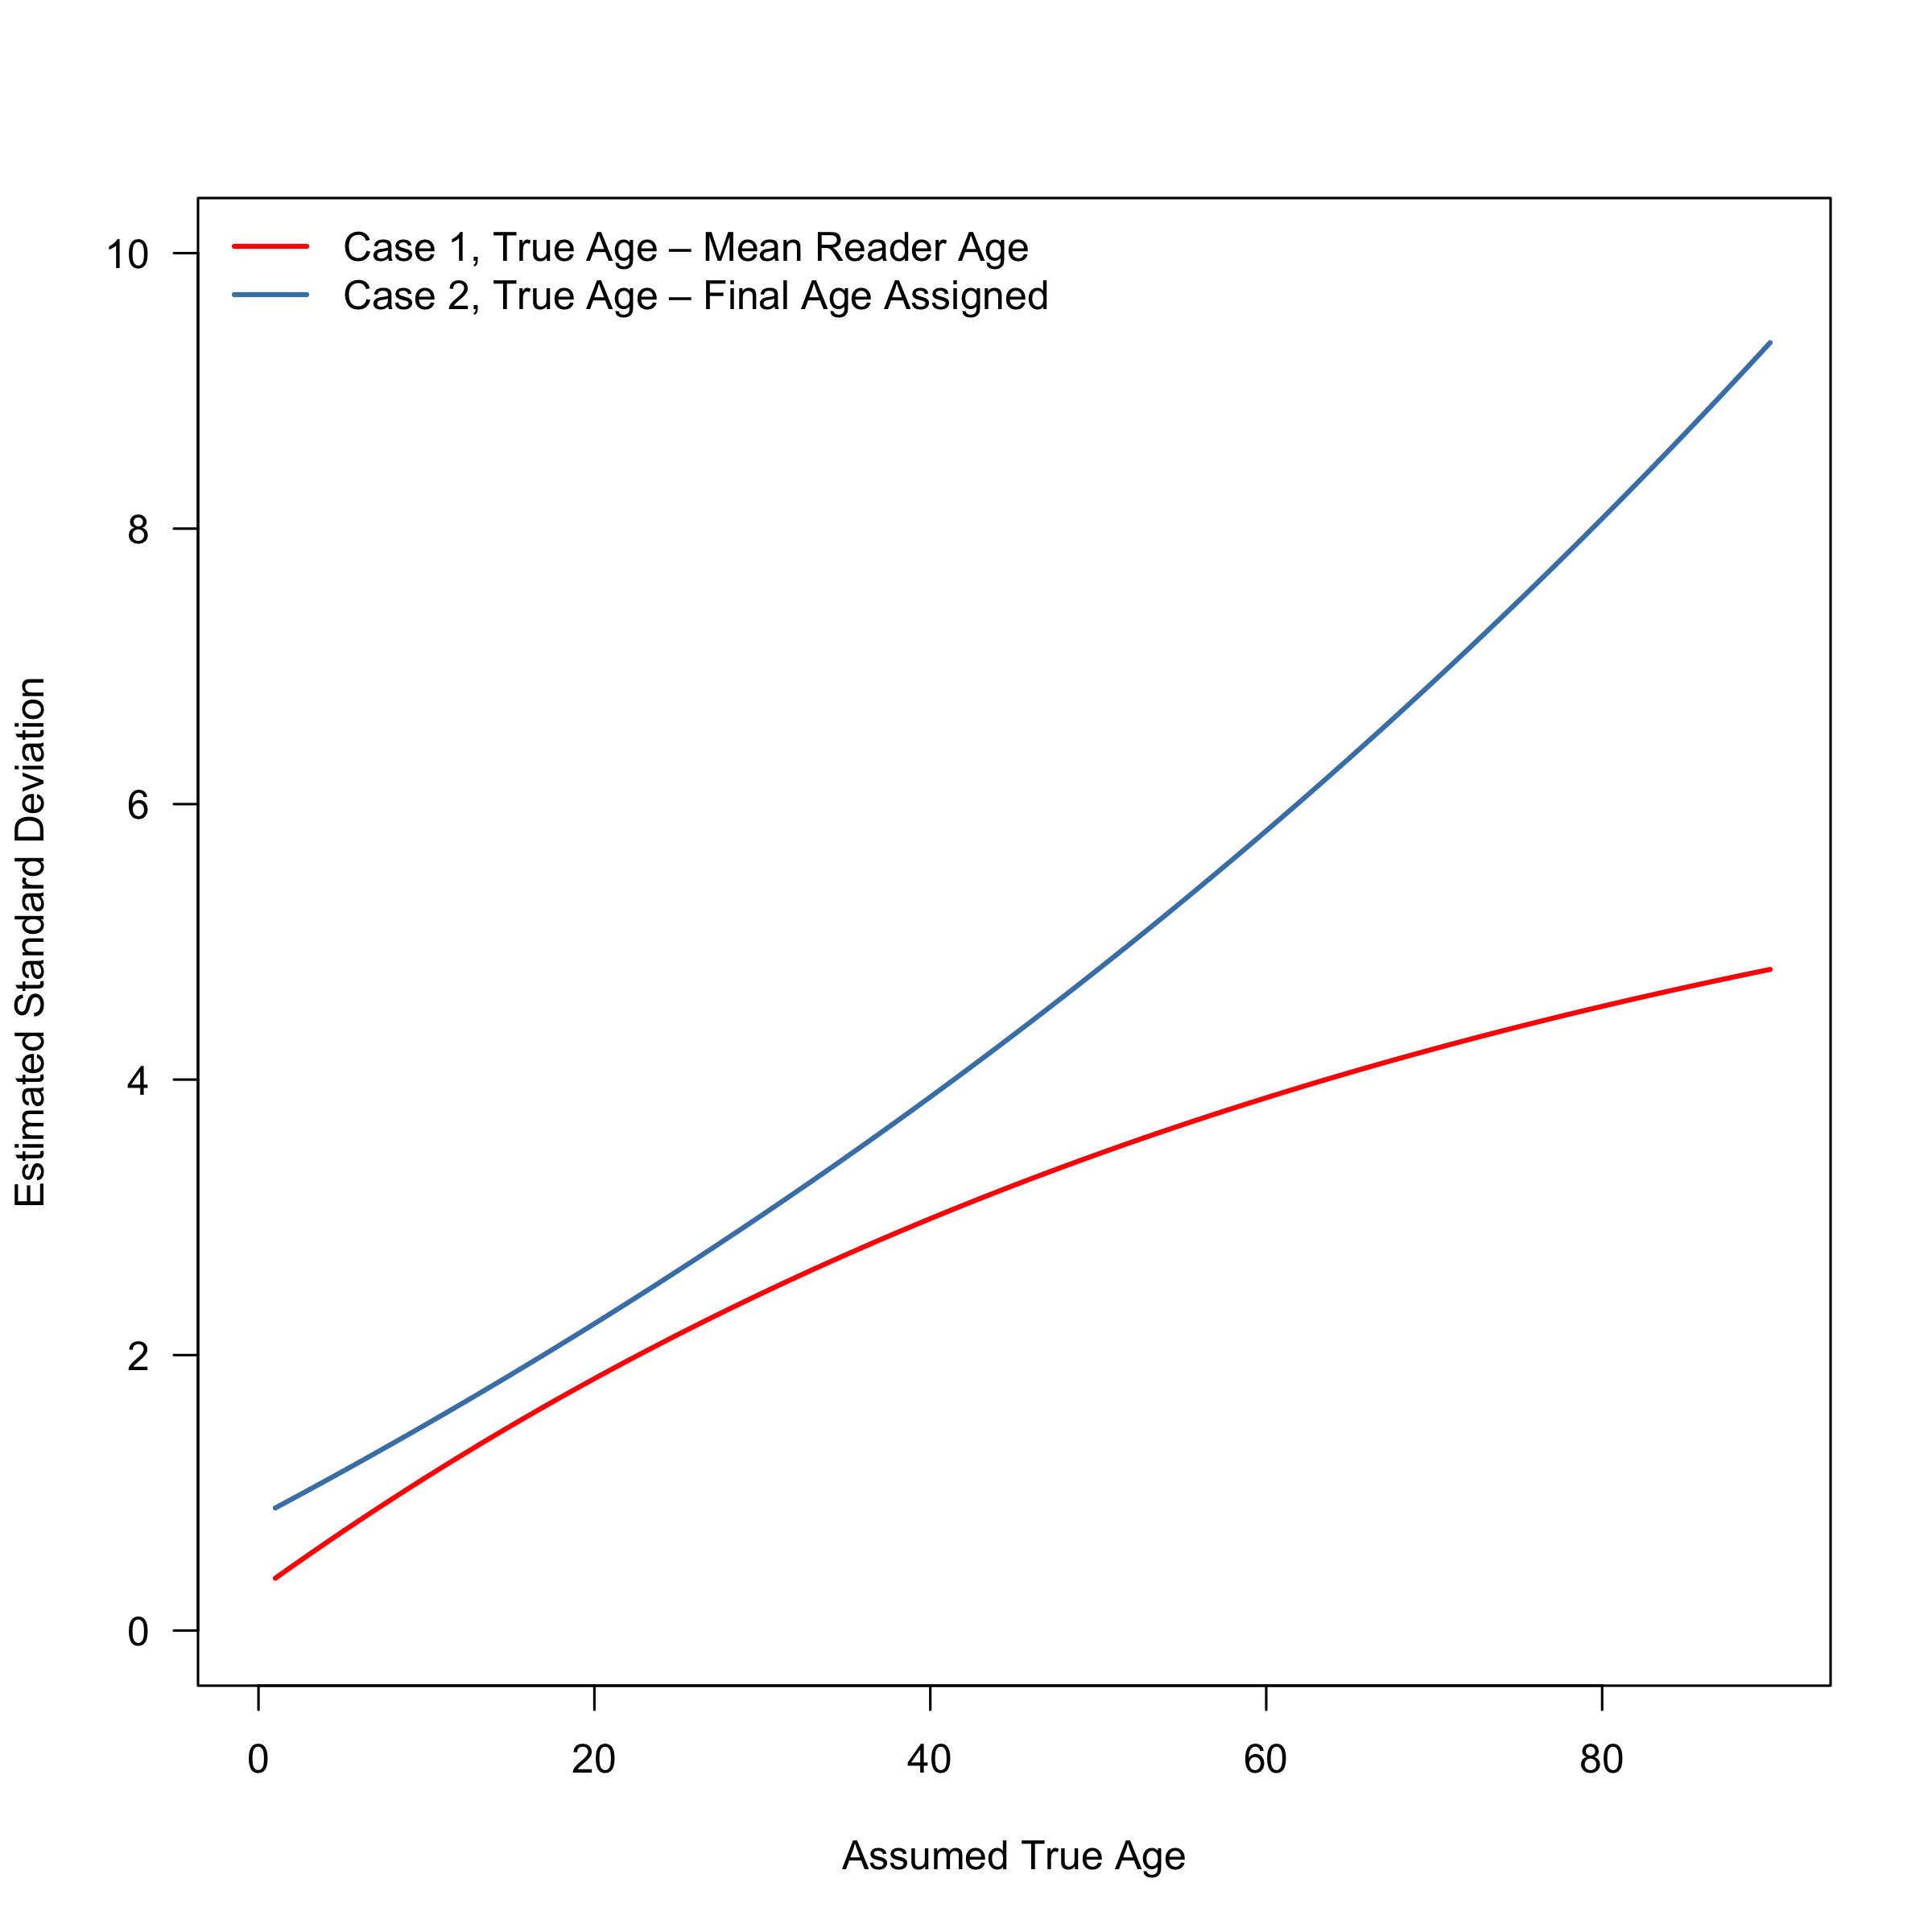
\includegraphics[width=0.9\linewidth]{data/ageErr1}}{Figure \ref{fig:unnamed-chunk-5}} 

}

\caption{Estimated standard deviation of observed ages for the two cases considered..}\label{fig:unnamed-chunk-5}
\end{figure}
\newpage
\begin{figure}[htb]

{\centering \pdftooltip{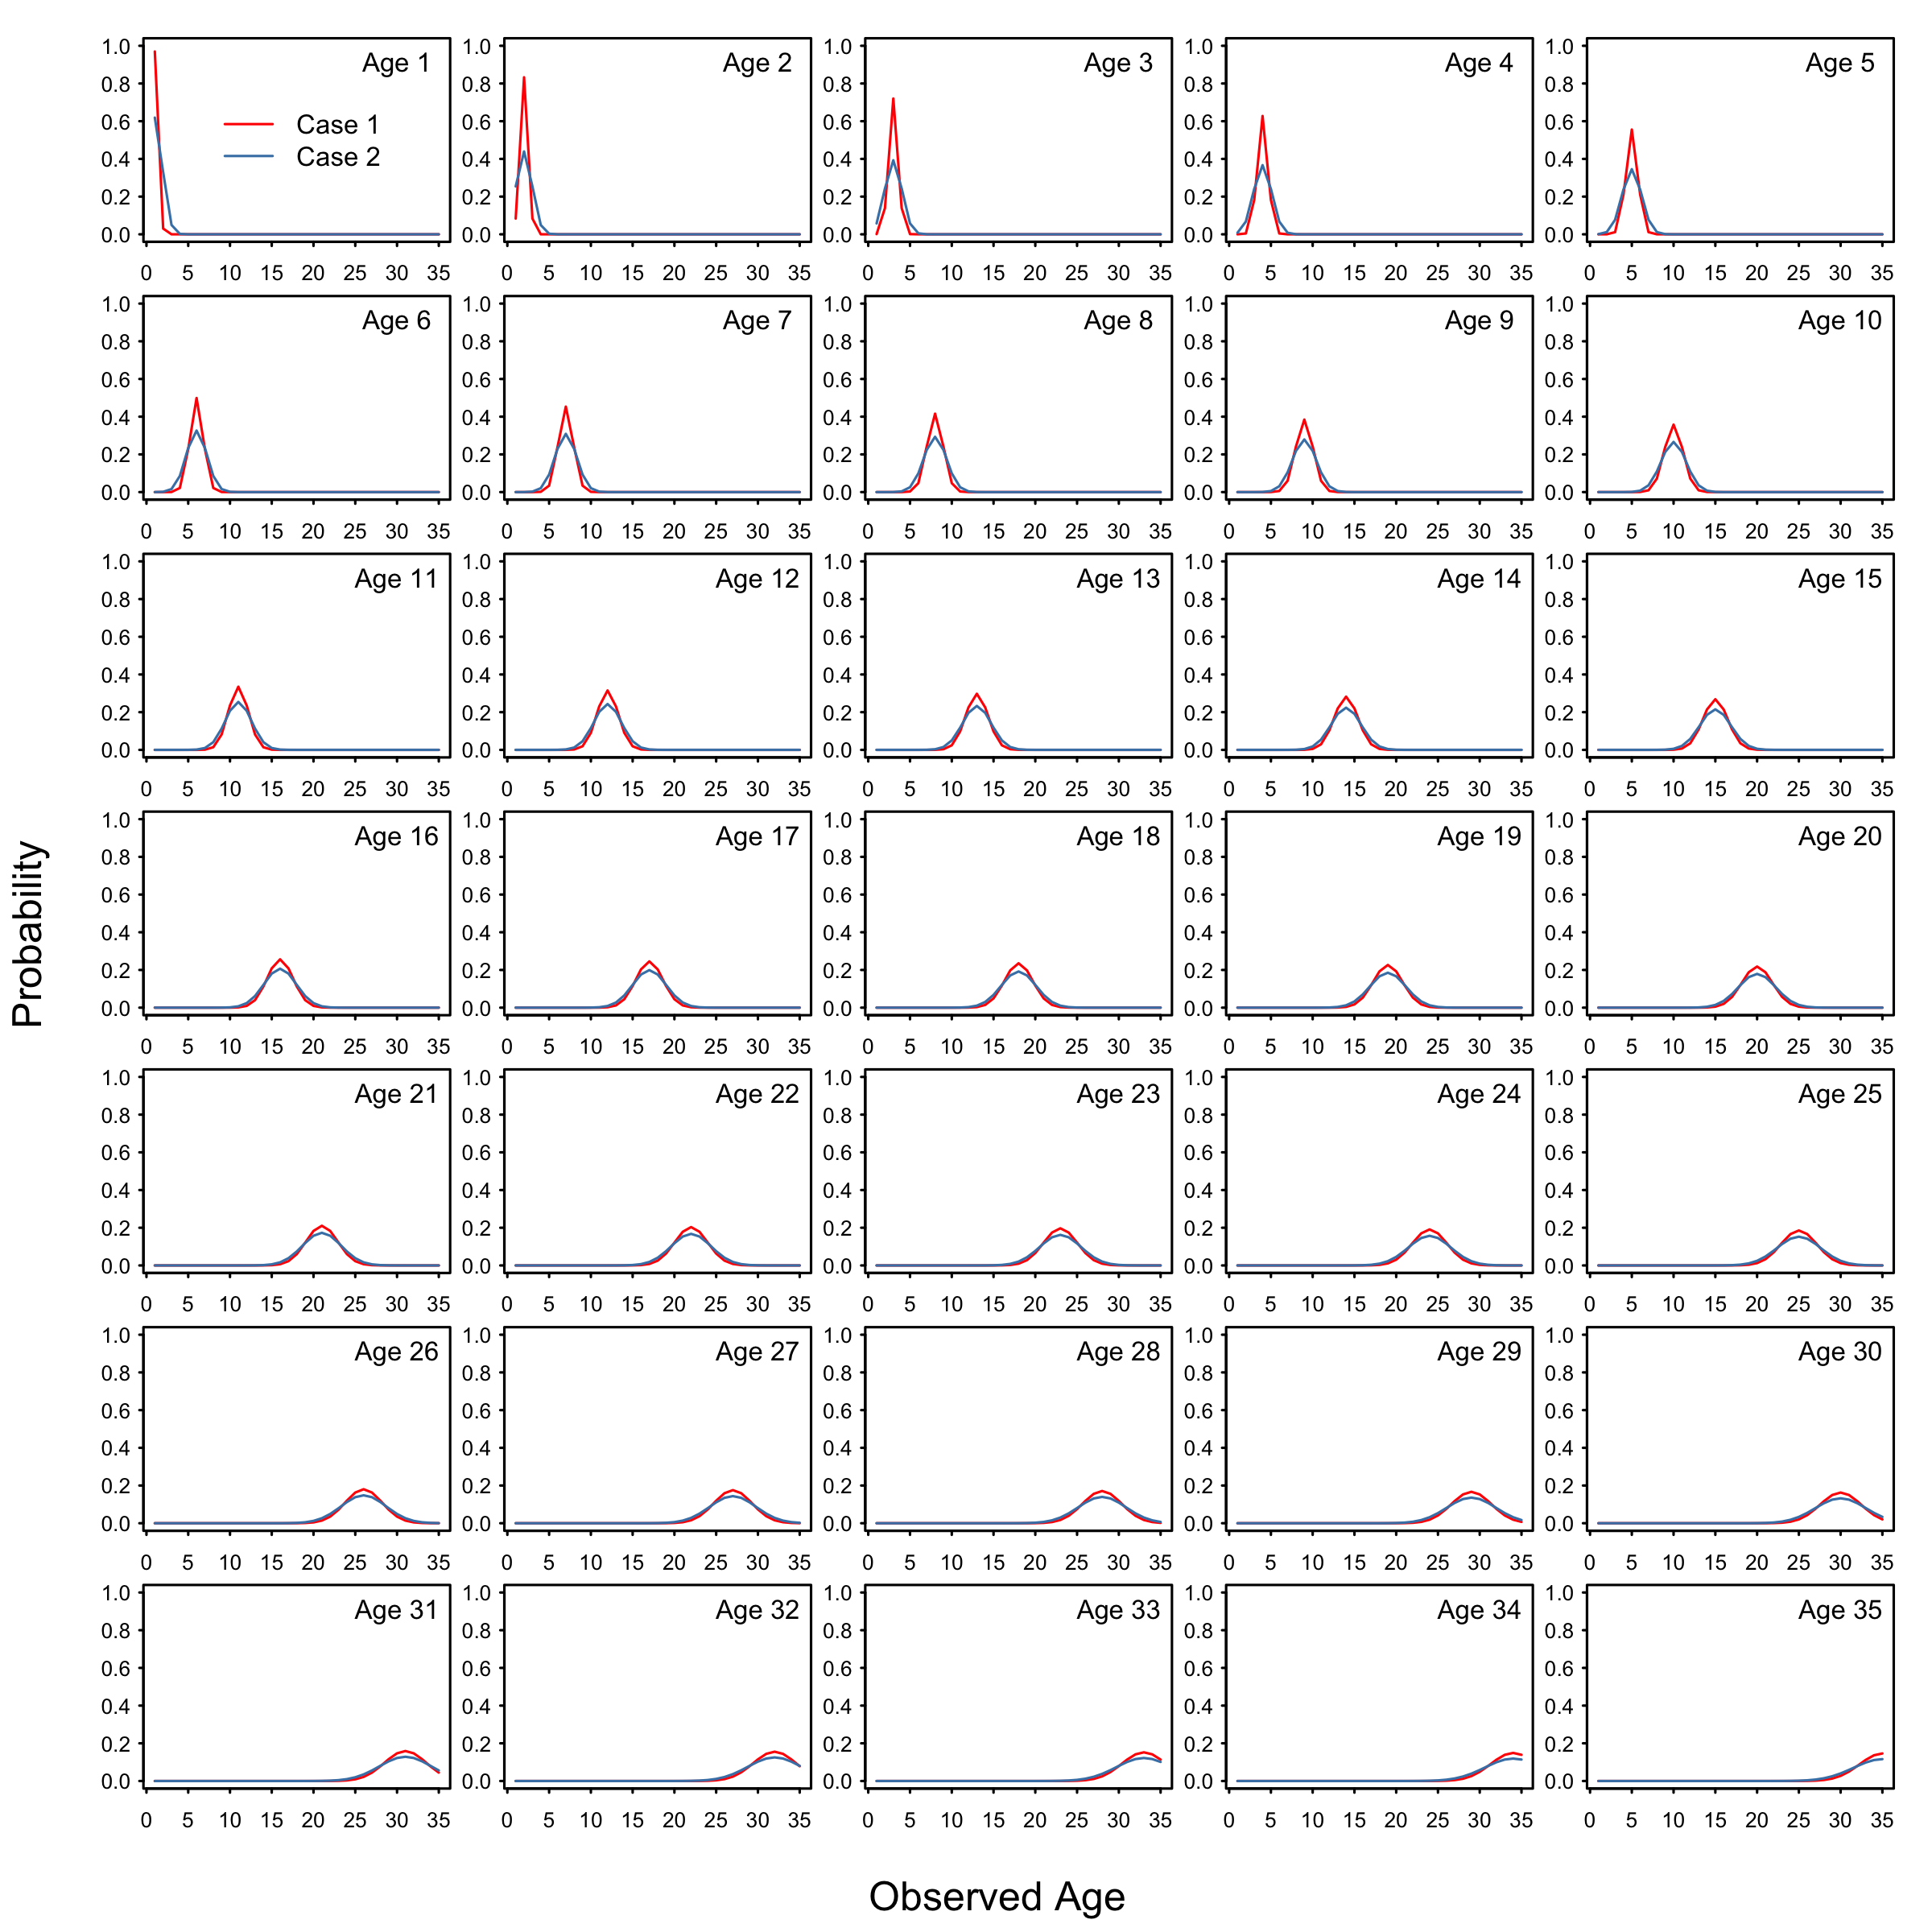
\includegraphics[width=0.9\linewidth]{data/ageErr2}}{Figure \ref{fig:unnamed-chunk-6}} 

}

\caption{Probability of observed ages given the true age indicated in top right corner of each plot for both cases considered.}\label{fig:unnamed-chunk-6}
\end{figure}
\hypertarget{refs}{}
\leavevmode\hypertarget{ref-hanselman2012statistical}{}%
Hanselman, D.H., Clark, W.G., Heifetz, J., and Anderl, D.M. 2012. Statistical distribution of age readings of known-age sablefish (anoplopoma fimbria). Fisheries Research 131: 1--8. Elsevier.

\leavevmode\hypertarget{ref-heifetz1999age}{}%
Heifetz, J., Anderl, D., Maloney, N., and Rutecki, T. 1999. Age validation and analysis of ageing error from marked and recaptured sablefish, anoplopoma fimbria. FISHERY BULLETIN-NATIONAL OCEANIC AND ATMOSPHERIC ADMINISTRATION 97: 256--263. SCIENTIFIC PUBLICATIONS OFFICE.

\leavevmode\hypertarget{ref-lai1987effects}{}%
Lai, H.L., and Gunderson, D.R. 1987. Effects of ageing errors on estimates of growth, mortality and yield per recruit for walleye pollock (theragra chalcogramma). Fisheries Research 5(2-3): 287--302. Elsevier.

\leavevmode\hypertarget{ref-richards1992statistical}{}%
Richards, L.J., Schnute, J.T., Kronlund, A., and Beamish, R.J. 1992. Statistical models for the analysis of ageing error. Canadian Journal of Fisheries and Aquatic Sciences 49(9): 1801--1815. NRC Research Press.

\leavevmode\hypertarget{ref-tyler1989implications}{}%
Tyler, A., Beamish, R., and McFarlane, G. 1989. Implications of age determination errors to yield estimates. Canadian Special Publication of Fisheries and Aquatic Sciences 108: 27--35.

\MakeAvailable

\end{document}
